\leftsection{Программа 1}

\subsection{Однопоточная программа}

\begin{lstlisting}[language=c, caption={Первая программа (однопоточный вариант)}]
#include <stdlib.h>
#include <stdio.h>
#include <fcntl.h>
#include <unistd.h>

#define MAX_FDS 10
#define MAX_BUF_SIZE 100

struct arg
{
    int valid;
    size_t amount;
    size_t buf_size;
};

int main(int argc, char **argv)
{
    const struct arg arg = parse_args(argc, argv);

    if (EXIT_SUCCESS != arg.valid)
        return EXIT_FAILURE;

    FILE *fds[MAX_FDS] = {NULL};
    char buf[MAX_FDS][MAX_BUF_SIZE], c;
    int fd = open("alphabet", O_RDONLY), rc = EXIT_SUCCESS;

    if (0 > fd)
    {
        perror("open error\n");
        rc = EXIT_FAILURE;
    }

    for (size_t i = 0; EXIT_SUCCESS == rc && arg.amount > i; i++)
    {
        fds[i] = fdopen(fd, "r");

        if (!fds[i])
        {
            perror("fdopen error\n");
            rc = EXIT_FAILURE;
        }
        else if (EXIT_SUCCESS
                 != setvbuf(fds[i], buf[i], _IOFBF, arg.buf_size))
        {
            perror("setvbuf error\n");
            rc = EXIT_FAILURE;
        }
    }

    if (EXIT_SUCCESS == rc)
        for (int r = 1; r && !(r = 0);)
            for (size_t i = 0; arg.amount > i; i++)
                if (1 == fscanf(fds[i], "%c", &c))
                {
                    fprintf(stdout, "%c\n", c);
                    r = 1;
                }

    for (size_t i = 0; arg.amount > i; i++)
        if (fds[i])
            fclose(fds[i]);

    if (0 <= fd)
        close(fd);

    return rc;
}
\end{lstlisting}

\clearpage

\begin{figure}[h]
    \centering
    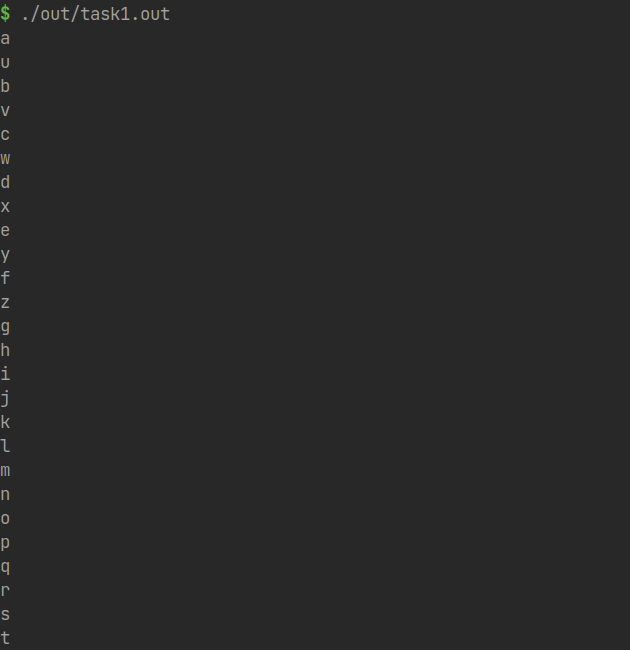
\includegraphics[width=0.7\textwidth]{task1.png}
    \caption{Результат работы первой программы}
\end{figure}

В результате работы описанной выше программы можно видеть, что при работе со
вторым файловым дескриптором вывод начинается с символа <<u>> (20 в алфавите),
что происходит из-за наличия буфера. При первом вызове fscanf в буфер первого
файлового дескриптора считываются 20 символов, второго --- оставшиеся 6.

\subsection{Многопоточная программа}

\begin{lstlisting}[language=c, caption={Первая программа (многопоточный вариант)}]
#include <stdlib.h>
#include <stdio.h>
#include <fcntl.h>
#include <unistd.h>
#include <pthread.h>

#define MAX_THREADS  12
#define MAX_BUF_SIZE 200

struct data
{
    int valid;
    size_t threads;
    size_t buf_size;
    int fd;
};

struct handle
{
    size_t id;
    const struct data *data;
};

void *thread_func(void *_arg)
{
    struct handle *arg = _arg;
    char buf[MAX_BUF_SIZE], tmp;
    int rc = EXIT_SUCCESS;

    FILE *f = fdopen(arg->data->fd, "r");

    if (!f)
    {
        perror("fdopen error\n");
        rc = EXIT_FAILURE;
    }
    else if (EXIT_SUCCESS != setvbuf(f, buf, _IOFBF, arg->data->buf_size))
    {
        perror("setvbuf error\n");
        rc = EXIT_FAILURE;
    }

    if (EXIT_SUCCESS == rc)
        for (int read = 1; read;)
            if ((read = (1 == fscanf(f, "%c", &tmp))))
                fprintf(stdout, "thread %zu: %c\n", arg->id, tmp);

    if (f)
        fclose(f);

    return NULL;
}

int main(int argc, char **argv)
{
    struct data data = parse_args(argc, argv);

    if (EXIT_SUCCESS != data.valid)
        return EXIT_FAILURE;

    struct handle args[MAX_THREADS];
    pthread_t threads[MAX_THREADS];

    int rc = EXIT_SUCCESS;
    data.fd = open("alphabet", O_RDONLY);

    if (0 > data.fd)
    {
        perror("open error\n");
        rc = EXIT_FAILURE;
    }

    for (size_t i = 0; EXIT_SUCCESS == rc && data.threads > i; i++)
    {
        args[i].id = i + 1;
        args[i].data = &data;

        if (EXIT_SUCCESS
            != pthread_create(threads + i, NULL, thread_func, args + i))
        {
            perror("pthread_create error\n");
            rc = EXIT_FAILURE;
        }
    }

    for (size_t i = 0; data.threads > i; i++)
        pthread_join(threads[i], NULL);

    if (0 <= data.fd)
        close(data.fd);

    return rc;
}
\end{lstlisting}

\clearpage

\begin{figure}[h]
    \centering
    \hspace*{\fill}
    \begin{minipage}{0.4\textwidth}
        \centering
        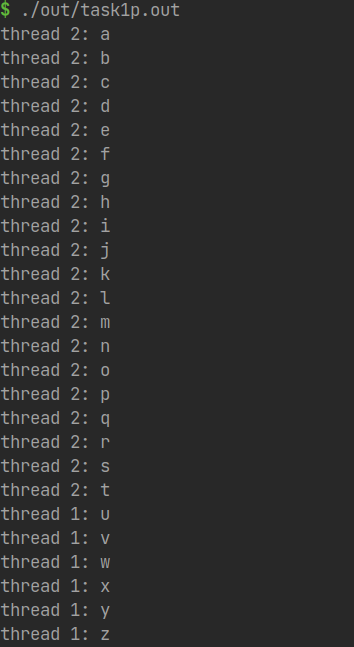
\includegraphics[width=\linewidth]{task1p1.png}
        Потоки: 2, Буфер: 20
    \end{minipage}
    \hfill
    \begin{minipage}{0.49\textwidth}
        \centering
        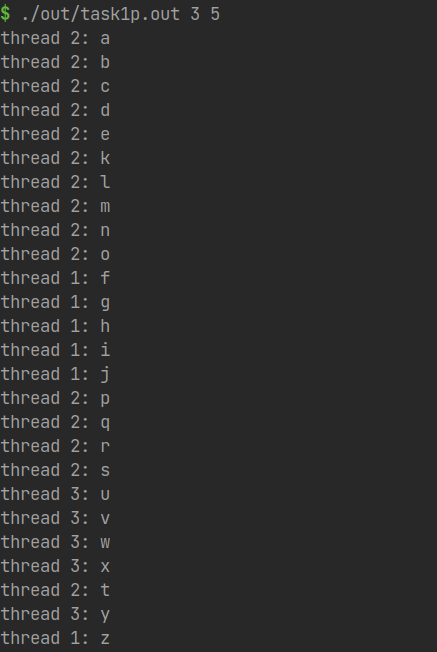
\includegraphics[width=\linewidth]{task1p2.png}
        Потоки: 3, Буфер: 5
    \end{minipage}
    \hspace*{\fill}
    \caption{Результат работы первой программы.}
\end{figure}

В многопоточном варианте программы чтение также буферизовано. Все потоки
считывают из файла количество байт, равное размеру буфера, а так как работа
потоков не синхронизирована, то и последовательность вывода нарушается.

\clearpage

\subsection{Связь структур}

\vspace*{\fill}
\begin{figure}[h]
    \centering
    \def\svgwidth{\textwidth}
    \leftsection{Программа 1}

\subsection{Однопоточная программа}

\begin{lstlisting}[language=c, caption={Первая программа (однопоточный вариант)}]
#include <stdlib.h>
#include <stdio.h>
#include <fcntl.h>
#include <unistd.h>

#define MAX_FDS 10
#define MAX_BUF_SIZE 100

struct arg
{
    int valid;
    size_t amount;
    size_t buf_size;
};

int main(int argc, char **argv)
{
    const struct arg arg = parse_args(argc, argv);

    if (EXIT_SUCCESS != arg.valid)
        return EXIT_FAILURE;

    FILE *fds[MAX_FDS] = {NULL};
    char buf[MAX_FDS][MAX_BUF_SIZE], c;
    int fd = open("alphabet", O_RDONLY), rc = EXIT_SUCCESS;

    if (0 > fd)
    {
        perror("open error\n");
        rc = EXIT_FAILURE;
    }

    for (size_t i = 0; EXIT_SUCCESS == rc && arg.amount > i; i++)
    {
        fds[i] = fdopen(fd, "r");

        if (!fds[i])
        {
            perror("fdopen error\n");
            rc = EXIT_FAILURE;
        }
        else if (EXIT_SUCCESS
                 != setvbuf(fds[i], buf[i], _IOFBF, arg.buf_size))
        {
            perror("setvbuf error\n");
            rc = EXIT_FAILURE;
        }
    }

    if (EXIT_SUCCESS == rc)
        for (int r = 1; r && !(r = 0);)
            for (size_t i = 0; arg.amount > i; i++)
                if (1 == fscanf(fds[i], "%c", &c))
                {
                    fprintf(stdout, "%c\n", c);
                    r = 1;
                }

    for (size_t i = 0; arg.amount > i; i++)
        if (fds[i])
            fclose(fds[i]);

    if (0 <= fd)
        close(fd);

    return rc;
}
\end{lstlisting}

\clearpage

\begin{figure}[h]
    \centering
    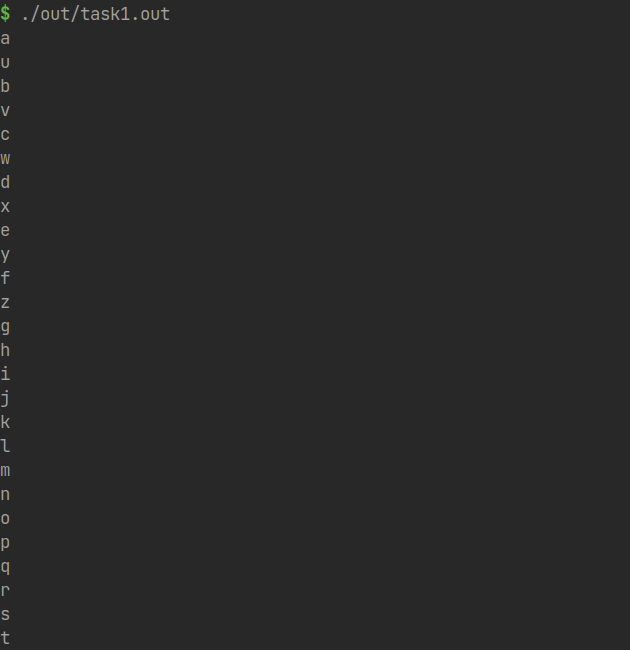
\includegraphics[width=0.7\textwidth]{task1.png}
    \caption{Результат работы первой программы}
\end{figure}

В результате работы описанной выше программы можно видеть, что при работе со
вторым файловым дескриптором вывод начинается с символа <<u>> (20 в алфавите),
что происходит из-за наличия буфера. При первом вызове fscanf в буфер первого
файлового дескриптора считываются 20 символов, второго --- оставшиеся 6.

\subsection{Многопоточная программа}

\begin{lstlisting}[language=c, caption={Первая программа (многопоточный вариант)}]
#include <stdlib.h>
#include <stdio.h>
#include <fcntl.h>
#include <unistd.h>
#include <pthread.h>

#define MAX_THREADS  12
#define MAX_BUF_SIZE 200

struct data
{
    int valid;
    size_t threads;
    size_t buf_size;
    int fd;
};

struct handle
{
    size_t id;
    const struct data *data;
};

void *thread_func(void *_arg)
{
    struct handle *arg = _arg;
    char buf[MAX_BUF_SIZE], tmp;
    int rc = EXIT_SUCCESS;

    FILE *f = fdopen(arg->data->fd, "r");

    if (!f)
    {
        perror("fdopen error\n");
        rc = EXIT_FAILURE;
    }
    else if (EXIT_SUCCESS != setvbuf(f, buf, _IOFBF, arg->data->buf_size))
    {
        perror("setvbuf error\n");
        rc = EXIT_FAILURE;
    }

    if (EXIT_SUCCESS == rc)
        for (int read = 1; read;)
            if ((read = (1 == fscanf(f, "%c", &tmp))))
                fprintf(stdout, "thread %zu: %c\n", arg->id, tmp);

    if (f)
        fclose(f);

    return NULL;
}

int main(int argc, char **argv)
{
    struct data data = parse_args(argc, argv);

    if (EXIT_SUCCESS != data.valid)
        return EXIT_FAILURE;

    struct handle args[MAX_THREADS];
    pthread_t threads[MAX_THREADS];

    int rc = EXIT_SUCCESS;
    data.fd = open("alphabet", O_RDONLY);

    if (0 > data.fd)
    {
        perror("open error\n");
        rc = EXIT_FAILURE;
    }

    for (size_t i = 0; EXIT_SUCCESS == rc && data.threads > i; i++)
    {
        args[i].id = i + 1;
        args[i].data = &data;

        if (EXIT_SUCCESS
            != pthread_create(threads + i, NULL, thread_func, args + i))
        {
            perror("pthread_create error\n");
            rc = EXIT_FAILURE;
        }
    }

    for (size_t i = 0; data.threads > i; i++)
        pthread_join(threads[i], NULL);

    if (0 <= data.fd)
        close(data.fd);

    return rc;
}
\end{lstlisting}

\clearpage

\begin{figure}[h]
    \centering
    \hspace*{\fill}
    \begin{minipage}{0.4\textwidth}
        \centering
        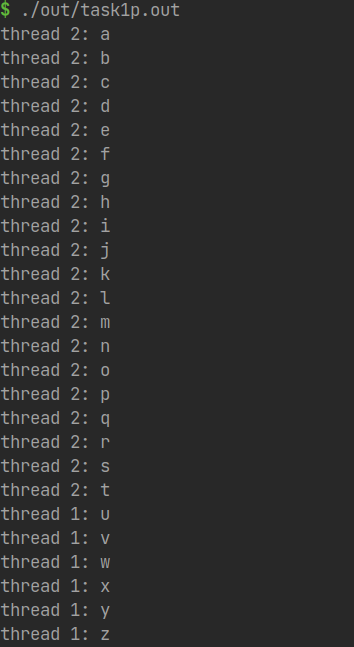
\includegraphics[width=\linewidth]{task1p1.png}
        Потоки: 2, Буфер: 20
    \end{minipage}
    \hfill
    \begin{minipage}{0.49\textwidth}
        \centering
        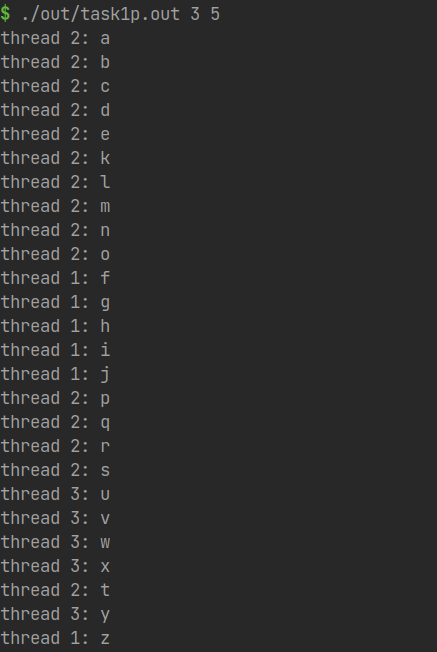
\includegraphics[width=\linewidth]{task1p2.png}
        Потоки: 3, Буфер: 5
    \end{minipage}
    \hspace*{\fill}
    \caption{Результат работы первой программы.}
\end{figure}

В многопоточном варианте программы чтение также буферизовано. Все потоки
считывают из файла количество байт, равное размеру буфера, а так как работа
потоков не синхронизирована, то и последовательность вывода нарушается.

\clearpage

\subsection{Связь структур}

\vspace*{\fill}
\begin{figure}[h]
    \centering
    \def\svgwidth{\textwidth}
    \leftsection{Программа 1}

\subsection{Однопоточная программа}

\begin{lstlisting}[language=c, caption={Первая программа (однопоточный вариант)}]
#include <stdlib.h>
#include <stdio.h>
#include <fcntl.h>
#include <unistd.h>

#define MAX_FDS 10
#define MAX_BUF_SIZE 100

struct arg
{
    int valid;
    size_t amount;
    size_t buf_size;
};

int main(int argc, char **argv)
{
    const struct arg arg = parse_args(argc, argv);

    if (EXIT_SUCCESS != arg.valid)
        return EXIT_FAILURE;

    FILE *fds[MAX_FDS] = {NULL};
    char buf[MAX_FDS][MAX_BUF_SIZE], c;
    int fd = open("alphabet", O_RDONLY), rc = EXIT_SUCCESS;

    if (0 > fd)
    {
        perror("open error\n");
        rc = EXIT_FAILURE;
    }

    for (size_t i = 0; EXIT_SUCCESS == rc && arg.amount > i; i++)
    {
        fds[i] = fdopen(fd, "r");

        if (!fds[i])
        {
            perror("fdopen error\n");
            rc = EXIT_FAILURE;
        }
        else if (EXIT_SUCCESS
                 != setvbuf(fds[i], buf[i], _IOFBF, arg.buf_size))
        {
            perror("setvbuf error\n");
            rc = EXIT_FAILURE;
        }
    }

    if (EXIT_SUCCESS == rc)
        for (int r = 1; r && !(r = 0);)
            for (size_t i = 0; arg.amount > i; i++)
                if (1 == fscanf(fds[i], "%c", &c))
                {
                    fprintf(stdout, "%c\n", c);
                    r = 1;
                }

    for (size_t i = 0; arg.amount > i; i++)
        if (fds[i])
            fclose(fds[i]);

    if (0 <= fd)
        close(fd);

    return rc;
}
\end{lstlisting}

\clearpage

\begin{figure}[h]
    \centering
    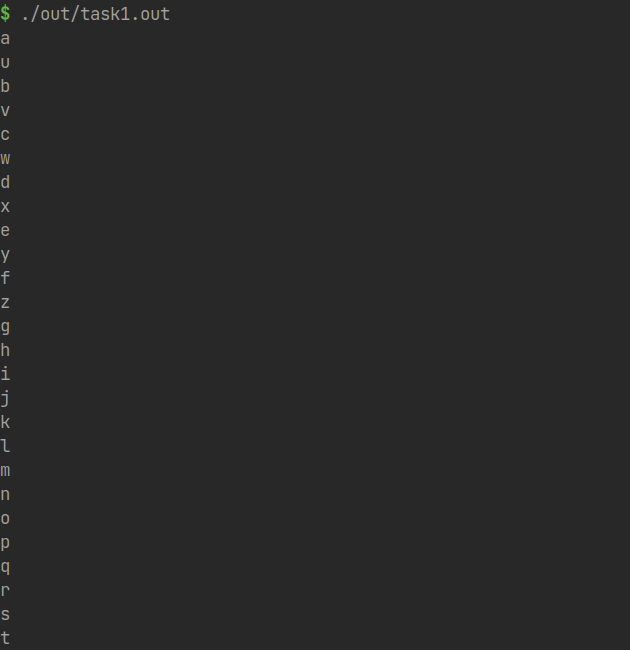
\includegraphics[width=0.7\textwidth]{task1.png}
    \caption{Результат работы первой программы}
\end{figure}

В результате работы описанной выше программы можно видеть, что при работе со
вторым файловым дескриптором вывод начинается с символа <<u>> (20 в алфавите),
что происходит из-за наличия буфера. При первом вызове fscanf в буфер первого
файлового дескриптора считываются 20 символов, второго --- оставшиеся 6.

\subsection{Многопоточная программа}

\begin{lstlisting}[language=c, caption={Первая программа (многопоточный вариант)}]
#include <stdlib.h>
#include <stdio.h>
#include <fcntl.h>
#include <unistd.h>
#include <pthread.h>

#define MAX_THREADS  12
#define MAX_BUF_SIZE 200

struct data
{
    int valid;
    size_t threads;
    size_t buf_size;
    int fd;
};

struct handle
{
    size_t id;
    const struct data *data;
};

void *thread_func(void *_arg)
{
    struct handle *arg = _arg;
    char buf[MAX_BUF_SIZE], tmp;
    int rc = EXIT_SUCCESS;

    FILE *f = fdopen(arg->data->fd, "r");

    if (!f)
    {
        perror("fdopen error\n");
        rc = EXIT_FAILURE;
    }
    else if (EXIT_SUCCESS != setvbuf(f, buf, _IOFBF, arg->data->buf_size))
    {
        perror("setvbuf error\n");
        rc = EXIT_FAILURE;
    }

    if (EXIT_SUCCESS == rc)
        for (int read = 1; read;)
            if ((read = (1 == fscanf(f, "%c", &tmp))))
                fprintf(stdout, "thread %zu: %c\n", arg->id, tmp);

    if (f)
        fclose(f);

    return NULL;
}

int main(int argc, char **argv)
{
    struct data data = parse_args(argc, argv);

    if (EXIT_SUCCESS != data.valid)
        return EXIT_FAILURE;

    struct handle args[MAX_THREADS];
    pthread_t threads[MAX_THREADS];

    int rc = EXIT_SUCCESS;
    data.fd = open("alphabet", O_RDONLY);

    if (0 > data.fd)
    {
        perror("open error\n");
        rc = EXIT_FAILURE;
    }

    for (size_t i = 0; EXIT_SUCCESS == rc && data.threads > i; i++)
    {
        args[i].id = i + 1;
        args[i].data = &data;

        if (EXIT_SUCCESS
            != pthread_create(threads + i, NULL, thread_func, args + i))
        {
            perror("pthread_create error\n");
            rc = EXIT_FAILURE;
        }
    }

    for (size_t i = 0; data.threads > i; i++)
        pthread_join(threads[i], NULL);

    if (0 <= data.fd)
        close(data.fd);

    return rc;
}
\end{lstlisting}

\clearpage

\begin{figure}[h]
    \centering
    \hspace*{\fill}
    \begin{minipage}{0.4\textwidth}
        \centering
        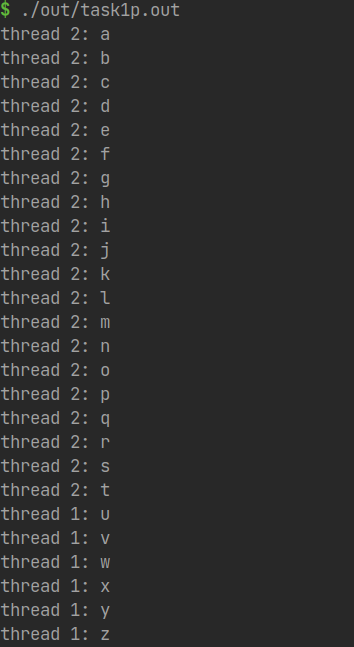
\includegraphics[width=\linewidth]{task1p1.png}
        Потоки: 2, Буфер: 20
    \end{minipage}
    \hfill
    \begin{minipage}{0.49\textwidth}
        \centering
        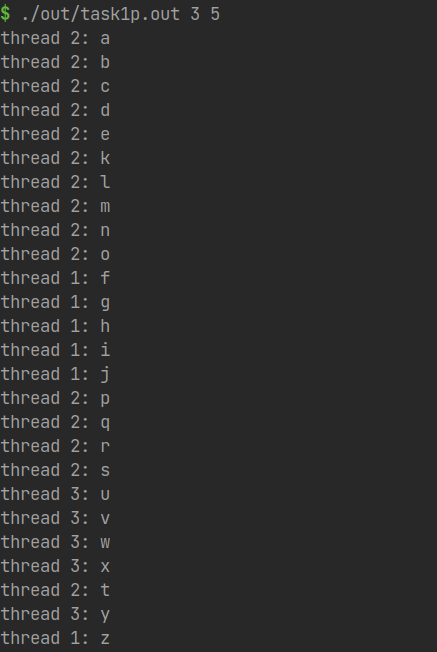
\includegraphics[width=\linewidth]{task1p2.png}
        Потоки: 3, Буфер: 5
    \end{minipage}
    \hspace*{\fill}
    \caption{Результат работы первой программы.}
\end{figure}

В многопоточном варианте программы чтение также буферизовано. Все потоки
считывают из файла количество байт, равное размеру буфера, а так как работа
потоков не синхронизирована, то и последовательность вывода нарушается.

\clearpage

\subsection{Связь структур}

\vspace*{\fill}
\begin{figure}[h]
    \centering
    \def\svgwidth{\textwidth}
    \leftsection{Программа 1}

\subsection{Однопоточная программа}

\begin{lstlisting}[language=c, caption={Первая программа (однопоточный вариант)}]
#include <stdlib.h>
#include <stdio.h>
#include <fcntl.h>
#include <unistd.h>

#define MAX_FDS 10
#define MAX_BUF_SIZE 100

struct arg
{
    int valid;
    size_t amount;
    size_t buf_size;
};

int main(int argc, char **argv)
{
    const struct arg arg = parse_args(argc, argv);

    if (EXIT_SUCCESS != arg.valid)
        return EXIT_FAILURE;

    FILE *fds[MAX_FDS] = {NULL};
    char buf[MAX_FDS][MAX_BUF_SIZE], c;
    int fd = open("alphabet", O_RDONLY), rc = EXIT_SUCCESS;

    if (0 > fd)
    {
        perror("open error\n");
        rc = EXIT_FAILURE;
    }

    for (size_t i = 0; EXIT_SUCCESS == rc && arg.amount > i; i++)
    {
        fds[i] = fdopen(fd, "r");

        if (!fds[i])
        {
            perror("fdopen error\n");
            rc = EXIT_FAILURE;
        }
        else if (EXIT_SUCCESS
                 != setvbuf(fds[i], buf[i], _IOFBF, arg.buf_size))
        {
            perror("setvbuf error\n");
            rc = EXIT_FAILURE;
        }
    }

    if (EXIT_SUCCESS == rc)
        for (int r = 1; r && !(r = 0);)
            for (size_t i = 0; arg.amount > i; i++)
                if (1 == fscanf(fds[i], "%c", &c))
                {
                    fprintf(stdout, "%c\n", c);
                    r = 1;
                }

    for (size_t i = 0; arg.amount > i; i++)
        if (fds[i])
            fclose(fds[i]);

    if (0 <= fd)
        close(fd);

    return rc;
}
\end{lstlisting}

\clearpage

\begin{figure}[h]
    \centering
    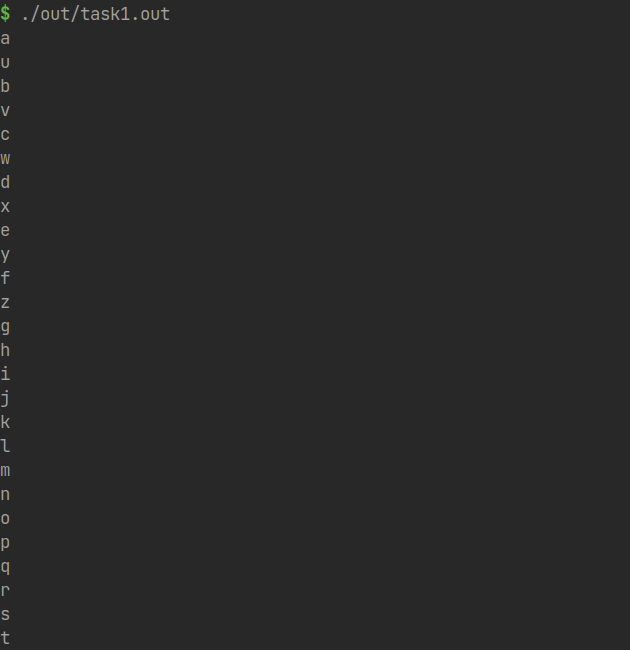
\includegraphics[width=0.7\textwidth]{task1.png}
    \caption{Результат работы первой программы}
\end{figure}

В результате работы описанной выше программы можно видеть, что при работе со
вторым файловым дескриптором вывод начинается с символа <<u>> (20 в алфавите),
что происходит из-за наличия буфера. При первом вызове fscanf в буфер первого
файлового дескриптора считываются 20 символов, второго --- оставшиеся 6.

\subsection{Многопоточная программа}

\begin{lstlisting}[language=c, caption={Первая программа (многопоточный вариант)}]
#include <stdlib.h>
#include <stdio.h>
#include <fcntl.h>
#include <unistd.h>
#include <pthread.h>

#define MAX_THREADS  12
#define MAX_BUF_SIZE 200

struct data
{
    int valid;
    size_t threads;
    size_t buf_size;
    int fd;
};

struct handle
{
    size_t id;
    const struct data *data;
};

void *thread_func(void *_arg)
{
    struct handle *arg = _arg;
    char buf[MAX_BUF_SIZE], tmp;
    int rc = EXIT_SUCCESS;

    FILE *f = fdopen(arg->data->fd, "r");

    if (!f)
    {
        perror("fdopen error\n");
        rc = EXIT_FAILURE;
    }
    else if (EXIT_SUCCESS != setvbuf(f, buf, _IOFBF, arg->data->buf_size))
    {
        perror("setvbuf error\n");
        rc = EXIT_FAILURE;
    }

    if (EXIT_SUCCESS == rc)
        for (int read = 1; read;)
            if ((read = (1 == fscanf(f, "%c", &tmp))))
                fprintf(stdout, "thread %zu: %c\n", arg->id, tmp);

    if (f)
        fclose(f);

    return NULL;
}

int main(int argc, char **argv)
{
    struct data data = parse_args(argc, argv);

    if (EXIT_SUCCESS != data.valid)
        return EXIT_FAILURE;

    struct handle args[MAX_THREADS];
    pthread_t threads[MAX_THREADS];

    int rc = EXIT_SUCCESS;
    data.fd = open("alphabet", O_RDONLY);

    if (0 > data.fd)
    {
        perror("open error\n");
        rc = EXIT_FAILURE;
    }

    for (size_t i = 0; EXIT_SUCCESS == rc && data.threads > i; i++)
    {
        args[i].id = i + 1;
        args[i].data = &data;

        if (EXIT_SUCCESS
            != pthread_create(threads + i, NULL, thread_func, args + i))
        {
            perror("pthread_create error\n");
            rc = EXIT_FAILURE;
        }
    }

    for (size_t i = 0; data.threads > i; i++)
        pthread_join(threads[i], NULL);

    if (0 <= data.fd)
        close(data.fd);

    return rc;
}
\end{lstlisting}

\clearpage

\begin{figure}[h]
    \centering
    \hspace*{\fill}
    \begin{minipage}{0.4\textwidth}
        \centering
        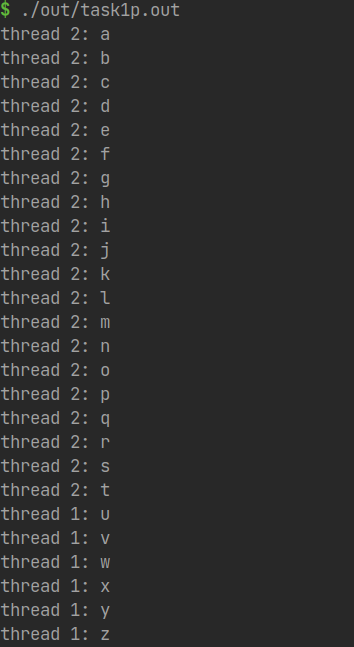
\includegraphics[width=\linewidth]{task1p1.png}
        Потоки: 2, Буфер: 20
    \end{minipage}
    \hfill
    \begin{minipage}{0.49\textwidth}
        \centering
        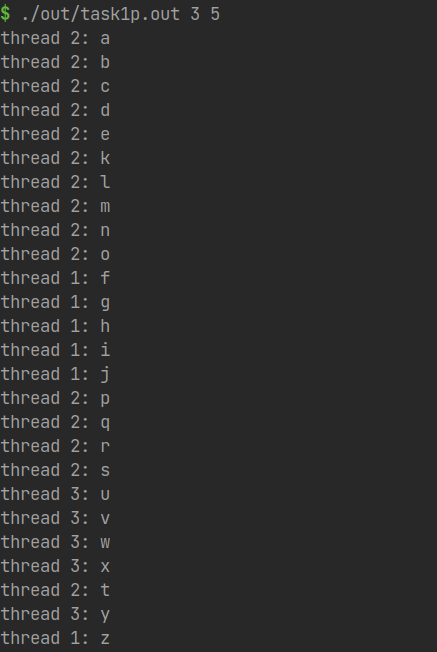
\includegraphics[width=\linewidth]{task1p2.png}
        Потоки: 3, Буфер: 5
    \end{minipage}
    \hspace*{\fill}
    \caption{Результат работы первой программы.}
\end{figure}

В многопоточном варианте программы чтение также буферизовано. Все потоки
считывают из файла количество байт, равное размеру буфера, а так как работа
потоков не синхронизирована, то и последовательность вывода нарушается.

\clearpage

\subsection{Связь структур}

\vspace*{\fill}
\begin{figure}[h]
    \centering
    \def\svgwidth{\textwidth}
    \input{task1.pdf_tex}
\end{figure}
\vfill


\end{figure}
\vfill


\end{figure}
\vfill


\end{figure}
\vfill

